
\chapter{Charge Ratio of Atmospheric Muons at IICHEP-Madurai}

As a part of the ICAL R\&D program, a magnetised detector (mini-ICAL)
with 10 layers of RPCs has been built and operational at IICHEP,
Madurai situated near the INO site. Being a scale-down model of the
ICAL detector, the mini-ICAL is beeing studied a the prototype of
the magnetised ICAL. This prototype is mainly built to study the
performance of electronics equipment in the presence of the magnetic
field and to test the event reconstruction algorithms.
The cosmic ray data collected by the
detector setup is also used to calculate the charge ratio $(R)$
of the number of $\mu+$ to $\mu-$ arriving at the Earth's surface.
The testing of the reconstruction algorithms is the motivation behind
this study. By comparing the result from cosmic ray data with extreme
air shower (EAS) simulation, this study signifies the ability of
the magnet in identifying the charge of the particle.
The cosmic muons are created at the upper atmosphere when high energy
primary cosmic rays interact with the air molecules.
As the primary cosmic rays are dominated by the positively charged
particles, the production of the positively charged mesons are
favoured. The measurement of the muon charge ratio can also be used
to improve the hadronic interaction models and for better neutrino
flux prediction.

\section{Detector Setup of mini-ICAL}
The mini-ICAL detector is consist of 11 layers of iron of size
4\,m\,$\times$\,4\,m\,$\times$\,5.6\,cm with the interlayer gap
of 4.5\,cm weighing at 85\,Ton. This makes the dimentions of this
prototype detector are 4\,m\,$\times$\,4\,m\,$\times$\,1.06\,m.
The detector setup is shown in the Figure~\ref{fig:miniICAL_Setup}
where the $X$-axis of the detector is making an angle of $10^\circ$
with the geographic north.
The iron layers in the mini-ICAL magnet is made of soft iron with
the additional chemical composition of C\,(0.015\%), Mn\,(0.37\%),
P\,(0.012\%), S\,(0.008\%), Si\,(0.188\%), Al\,(0.001\%), N\,(50\,ppm).
This soft iron has low carbon content which makes it strong enough
mechanically to support its own weight, but also allows it to have high
high permeability with knee point at $\sim$1.5\,T.
Each of the layer of iron is consists of several different tiles shown
in the Figure~\ref{fig:miniICAL_iron}.
\begin{figure}[h]
  \centering
  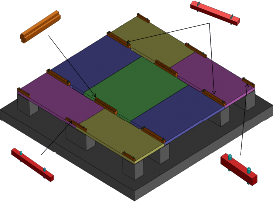
\includegraphics[width=0.75\linewidth]{miniICAL_iron_block.pdf} 
  \caption{One layer of iron of mini-ICAL Magnet}
  \label{fig:miniICAL_iron}
\end{figure}
The gap between the layers are maintained with the help of the spacers
made of non-magnetic stainless steel (SS-304) shown also in the
Figure~\ref{fig:miniICAL_iron}.

There are four slots with dimentions of 80\,cm\,$\times$\,8\,cm to
accommodate two sets of current conducting coils to create magnetic
field inside the iron in a similar fashion to the proposed
ICAL detector. The coils are made of OFE-grade copper with
oxygen content less than 10\,ppm. There are 18 turns of coils in each
set of coils. Each of the turns are kept at a distance of 40\,mm.
The coils are hollow inside with the cross section of
30\,mm\,$\times$\,30\,mm\,$\times$\,$\phi$17\,mm.
The two sets of coils are electrically connected in series,
and a low voltage power supply is used to supply 800\,Amp
of trough via the coils. An uniform magnetic field of $\sim$1.3\,T
is obtained in the central region of the detector. The magnetic field
in the mini-ICAL is along the (-)Y-direction in the central region.
The heat generated by the current in the
coils are extracted by a clossed-loop low conductivity water cooling
system (LCWCS) by flowing chilled water through the bore of the coils.

Ten RPCs of dimensions 174\,cm\,$\times$\,183.5\,cm are used as the
active detector. These RPCs are and placed in the central region of
the detector in between iron layers.
An RPC gap is made of two glass electrodes of thickness 3\,mm with
a gap of 2\,mm between them. Uniform gap between these two electrodes
is maintained using a array of 2\,mm thick poly-carbonate buttons.
The glass gap is sealed on the outer edges to make it air-tight.
A mixture of gases with the compositions of R134a (95.2\%),
iso-C$_4$H$_{10}$ (4.2\%) and SF$_6$ (0.3\%) is flown in the RPCs
via strategically placed nozzles. This mixture of gasses serves as the
target medium of the detector.
Both the outer surfaces of the glass gap are coated with a thin layer
of graphite. The RPCs are operated by applying a differential supply of
$\pm$\,5\,kV to the graphite layers which creates a constant electric
field between the glass electrodes. The ionisation of the gas mixture
by passage of the charged particles eventually evloves into a
avalanche in the presence of the high electric field between the glass
elctrodes. The avalanche in the RPCs induces signals in the two
orthogonal pickup panels placed on both sides of the glass gaps
labeled as X-side and Y-side. The pickup panels are made of parallel
copper strips of width 28\,mm with 2\,mm gap between two consecutive
strips. There are 58 strips on the X-side and 61 strips on the
Y-side for each layer.

The DAQ system is similar to the setup discussed in the previous
chapter. In this case the cosmic muon data have been collected using
the 1-Fold signals from top 4 layers as trigger.
An event data typically contains strip hit and timing information
of an event. The strip hit is basically one logic bit per strip
indicating the signal in that strip is above the threshold value
for that strip. The least count of each of the TDC is 0.1\,ns.
The timing data is consists of 16 time signal for
each layer where each multi-hit TDC channel records time signals
coming from every alternating 8$^{th}$ strips on one side of the layer.
The time signal of each hit is recorded for both the leading-edge and
the trailing-edge of the induced signal pulse.


\section{Monte-Carlo Simulation}
The Monte-Carlo Simulation for this study has been executed in
two stages. The Extensive Air Shower (EAS) has been simulated
by the CORSIKA simulation package\cite{corsika763}. The information
of daughter particles generated by the EAS at the earth's surface
level has been extracted and used as the input data to the detector
simulation. The detector simulation has been executed with the help
of the GEANT4 toolkit\cite{geant4}. The schemes of the EAS and the
detector simulations are already elaborated in the previous chapter.

Both the events from the observed cosmic ray data and the detector
simulation are reconstructed using the track fit algorithm which is
discussed in the next section.

\section{Event Reconstruction and Data Selection}
The recorded data is actually the projection of the track on the
\mbox{X--Z} and \mbox{Y--Z} planes. During the passage of a charged
particle through a RPC gap, the number of strips on which signal is
induced depends on the gain of the gas gap. This sharing of the induced
signal between the neighbouring strips is the main reason for the
observed strip multiplicity shown in the Figure~\ref{fig:layer2y}(c).
In order to prepare the events for analysis, the consecutive strips
which have recorded signal are clubbed together to form a cluster.
The layers with no clusters either or both on X and Y sides are
neglected during the track reconstruction.

Position resolutions of the clusters with more than one strip hit
are improved with the help of the Time-Over-Threashould (TOT). When a
signal is shared between two or more strips, the TOT for the strips in
the cluster depends on the actual position of the avalanche. Farther
the position of the avalanche from a strip, smaller the value of TOT
for that strip. So, observing the TOT of two strips (say, $T_{l}$
and $T_{r}$) at the both sides of a cluster can give valuable
information about the true position of the hit. The strip with the
lowest TOT value (say, $T_{l}$) is found, and also the deviation of
extrapolated position from the center of that strip (say, $\Delta x$).
Profile histograms have been created with the share of the TOT
$\left(=\frac{T_{l}}{T_{l}+T_{r}}\right)$ on the X-axis and the
deviation of extrapolated position from the middle of that strip
$\left(\Delta x\right)$ on the Y-axis. The profile histograms for 2
and 3 multiplicities in a layer are shown in the
Figure~\ref{fig:prof_tot}. With the help of these plots the position
resolutions are improved by 20\,\%.

%% During the study, the position resolution is calculated for different
%% strip multiplicities of 1, 2, 3, and 4 and the values observed are
%% $\sim$6\,mm, $\sim$8\,mm, $\sim$12\,mm and $\sim$22\,mm respectively.
%% The position resolutions for strip multiplicities more than four is
%% larger than the pitch of the strip (3\,cm).
%% In this study, the clusters of hits with more than 3 multiplicities are neglected as the position resolution for higher multiplicities is found to be the worse. A layer which has more than 15 strip hits and/or more than 10 clusters is tagged as `noisy layer' and not considered in the track reconstruction. An event which has more than 3 noisy layers is considered as `noisy event' and discarded.

Now, as it shown earlier, the strength of magnetic field in the
X-direction is very small. So, almost no significant bending is
observed in the Y-side of the track which makes the projection of
the track on the Y-side to be fit with a straight line.
Thus, in the first step of track reconstruction, the clusters on
the Y-side associated with the tracks are found and grouped using
the method of Hough Transformation\cite{hought}. This eliminates
the possibility of noise hits on the Y-side getting included in the
track reconstruction. Once one valid straight track found, attention
is given on the X-side of the track. As the magnetic field is mainly
in the Y-direction, maximum bending of track is observed on the X-side.
The clusters on the X-side is then fitted with a circle.
The information of the fitted circle helps to reject the noise hits
on the X-side as well.
Using the radius ($r$ in meter) of the fitted circle, the transverse
momentum ($p_t$ in GeV) of the particle can be roughly estimated by
the following equation,
\begin{equation}
  p_{t}=0.3Br \label{eq:pt_est}
\end{equation}
where, $B$ is the average magnetic field in Tesla.
The information of the fitted straight line on Y-side and the circle
on the X-side further used to calculate the direction (zenith and
azimuth) and the location of incidence of the particle roughly.

The momentum vector and the location of incidence, estimated
above are given as the input parameter to the track reconstruction.

%% There following representations of the equation of motion of a charged
%% particle moving through a magnetic field\cite{tracking} is choosen
%% for this case,
%% \begin{equation}
%%   \frac{d^{2}\vec{r}}{ds^{2}} = \frac{q}{p} \left(\frac{d\vec{r}}{ds} \times \vec{B}\left(\vec{r}\right)\right). \label{eq:eqmotion}
%% \end{equation}
%% The electric component of the Lorentz Force is ignored as it is
%% insignificant compared to the magnetic field. As the nature of the
%% magnetic field is not homogeneous in the detector, it is not possible
%% to find a solution analytically. It has to be solved numerically.
%% In this study, the Runge-Kutta-Nystr�m method have been integrated
%% in the track reconstruction to find the fit parameters\cite{tracking}.

%% A time-step of 5\,mm is used to propagate the particle in the
%% detector. At each step of the propagation the ionisation energy loss
%% of the particle is calculated using the graph shown in the
%% Figure~\ref{fig:eloss}.

The particle is propagated in the medium of the detector by integrating
the following equation numerically,
%% \begin{equation}
%%   \frac{\vec{F}}{q}=\vec{v}\times \vec{B} \label{eq:mom_force}
%% \end{equation}
\begin{equation}
  \vec{\ddot{x}} = \left(\frac{q}{\gamma m_{\mu}}\right)\vec{\dot{x}}\times \vec{B}
\end{equation}
where, $\vec{\dot{x}}=\frac{\vec{p}}{\gamma m_{\mu}}$ and
$\gamma=\sqrt{1+\left(\frac{p}{m_{\mu}c}\right)^{2}}$.

A time-step of 10\,ps is used to propagate the particle in the
detector. This is equivalent to a step-size of $\sim$3\,mm at speed
of light. At each step of the propagation the ionisation energy
loss of the particle is calculated using the graph shown in
the Figure~\ref{fig:eloss}.

The 5 parameters (3 momentum parameters and 2 position parameters) are
properly estimated by minimising the least-squared distance
($\chi^{2}$).
The exhaustive grid-search method have been adopted to minimised the
$\chi^{2}$ as the maximum number of data points available is only 10.
Any other methods are are avoided as the chances of minimising the
$\chi^{2}$ to a local minima is very high with smaller number of data
points.
